\chapter{Image acquisition and formation}


\section{Pinhole camera}

\begin{description}
    \item[Imaging device] \marginnote{Imaging device}
        Gathers the light reflected by 3D objects in a scene and creates a 2D representation of them.

    \item[Computer vision] \marginnote{Computer vision}
        Infer knowledge of the 3D scene from 2D digital images.
\end{description}

\begin{description}
    \item[Pinhole camera] \marginnote{Pinhole camera}
        Imaging device where the light passes through a small pinhole and hits the image plane.
        Geometrically, the image is obtained by drawing straight rays from the scene to the image plane passing through the pinhole.

        \begin{remark}
            Larger aperture size of the pinhole results in blurry images (circle of confusion), 
            while smaller aperture results in sharper images but requires longer exposure time (as less light passes through).
        \end{remark}

        \begin{remark}
            The pinhole camera is a good approximation of the geometry of the image formation mechanism of modern imaging devices.
        \end{remark}

        \begin{figure}[H]
            \begin{subfigure}{.4\textwidth}
                \centering
                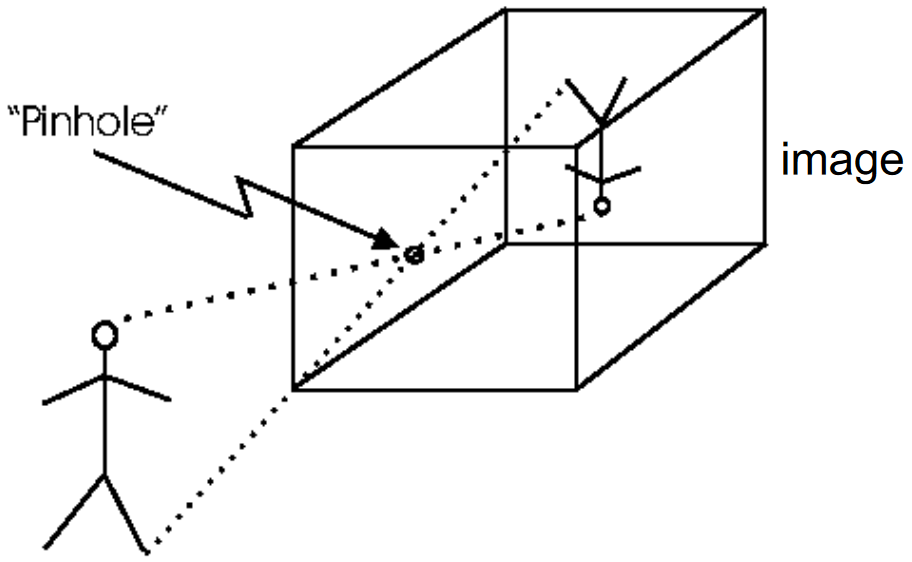
\includegraphics[width=0.8\linewidth]{./img/pinhole.png}
                \caption{Pinhole camera model}
            \end{subfigure}
            \begin{subfigure}{.45\textwidth}
                \centering
                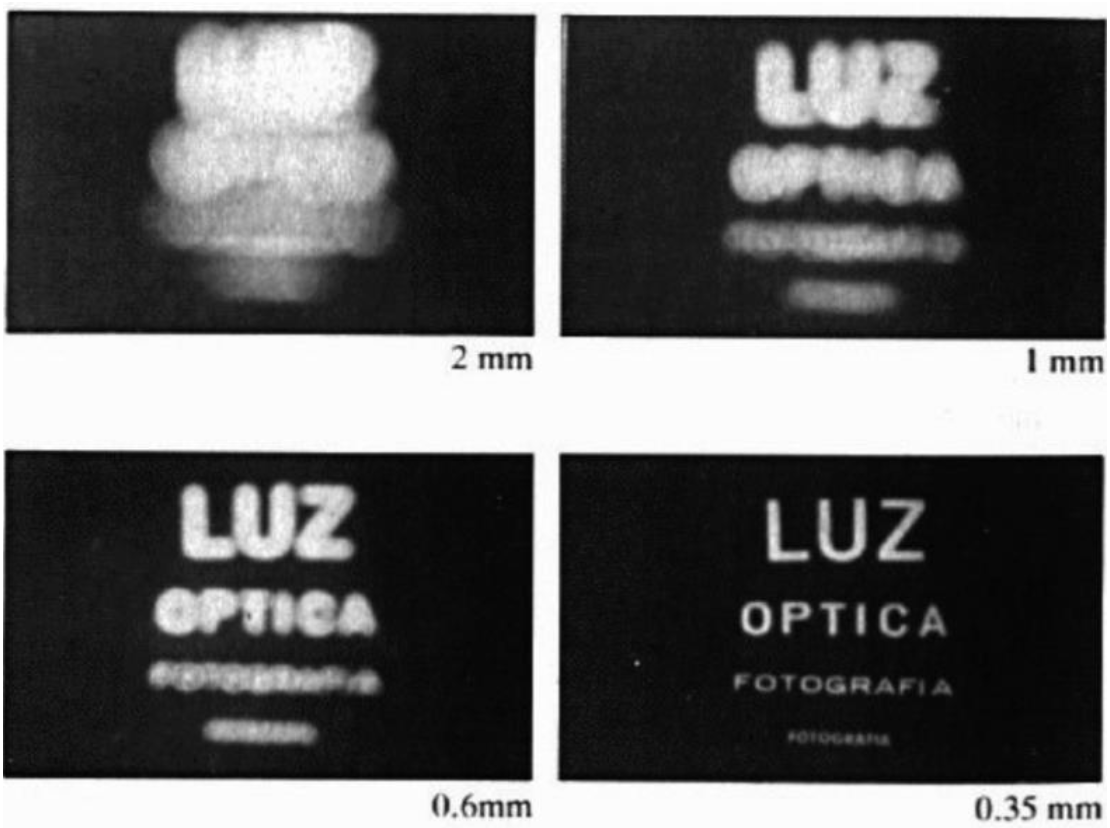
\includegraphics[width=0.7\linewidth]{./img/pinhole_hole_size.png}
                \caption{Images with varying pinhole aperture size}
            \end{subfigure}
        \end{figure}
\end{description}



\section{Perspective projection}
\marginnote{Perspective projection}

Geometric model of a pinhole camera.\\

\begin{minipage}{0.65\textwidth}
    \begin{description}
        \setlength\itemsep{0em}
        \item[Scene point] $M$ (the object in the real world).
        \item[Image point] $m$ (the object in the image).
        \item[Image plane] $I$.
        \item[Optical center] $C$ (the pinhole).
        \item[Image center/piercing point] $c$ (intersection between the optical axis -- the line orthogonal to $I$ passing through $C$ -- and $I$).
        \item[Focal length] $f$.
        \item[Focal plane] $F$.
    \end{description}
\end{minipage}
\begin{minipage}{0.3\textwidth}
    \centering
    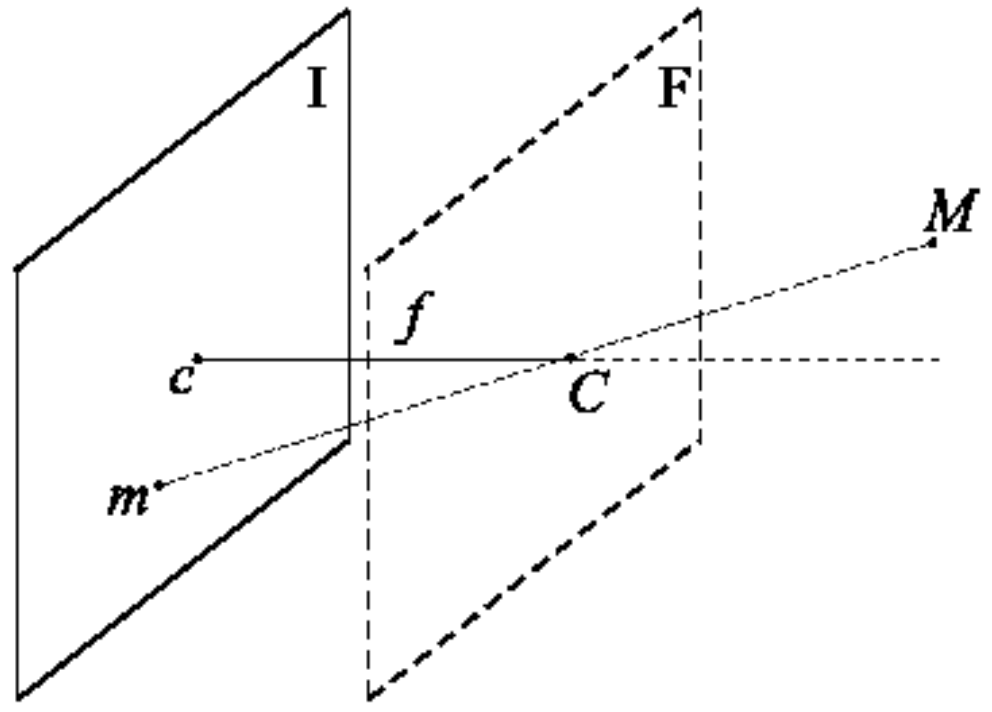
\includegraphics[width=\linewidth]{./img/perspective_projection1.png}
\end{minipage}\\

\begin{minipage}{0.55\textwidth}
    \begin{itemize}[leftmargin=*]
        \item $u$ and $v$ are the horizontal and vertical axis of the image plane, respectively.
        \item $x$ and $y$ are the horizontal and vertical axis of the 3D reference system, respectively, 
            and form the \textbf{camera reference system}. \marginnote{Camera reference system}
    \end{itemize}

    \begin{remark}
        For the perspective model, the coordinate systems $(U, V)$ and $(X, Y)$ must be parallel.
    \end{remark}
\end{minipage}
\begin{minipage}{0.35\textwidth}
    \centering
    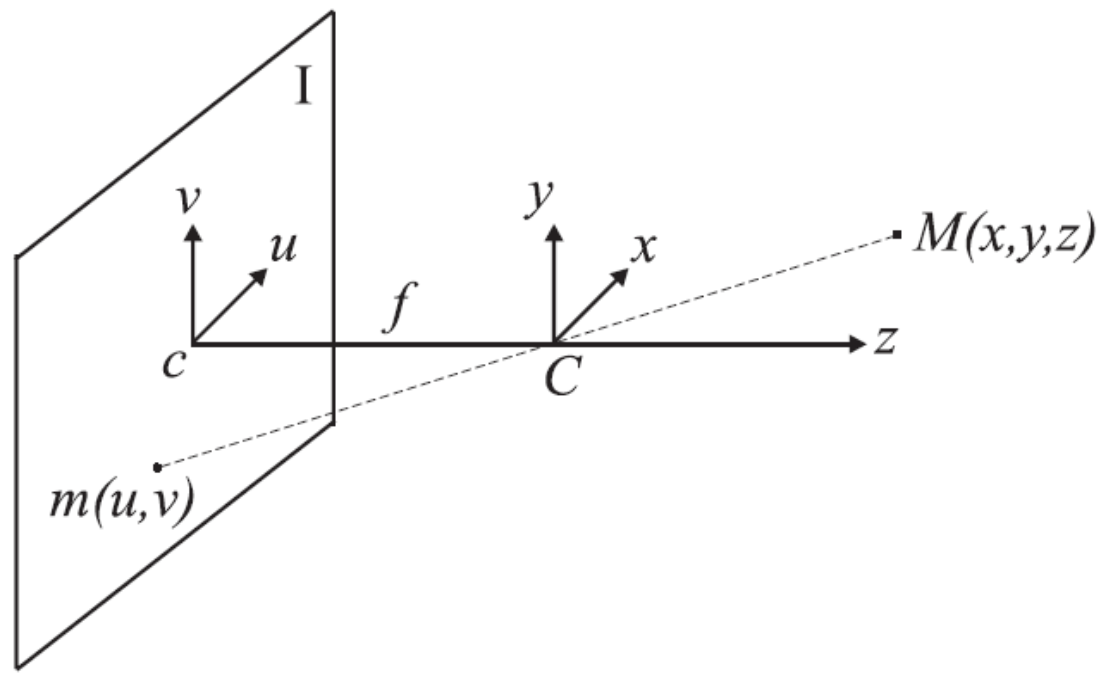
\includegraphics[width=\linewidth]{./img/perspective_projection2.png}
\end{minipage}

\begin{description}
    \item[Scene--image mapping] \marginnote{Scene--image mapping}
        The equations to map scene points into image points are the following:
        \[ u = x \frac{f}{z} \hspace*{3em} v = y \frac{f}{z} \]

        \begin{proof}
            This is the consequence of the triangle similarity theorems.

            \begin{minipage}{0.45\textwidth}
                \[ 
                    \begin{split}
                        \frac{u}{x} = -\frac{f}{z} &\iff u = -x \frac{f}{z} \\
                        \frac{v}{y} = -\frac{f}{z} &\iff v = -y \frac{f}{z} 
                    \end{split}
                \]
                The minus is needed as the axes are inverted
            \end{minipage}
            \begin{minipage}{0.50\textwidth}
                \begin{figure}[H]
                    \centering
                    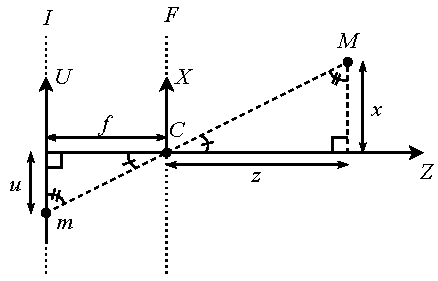
\includegraphics[width=0.7\textwidth]{./img/_perspective_projection_eq_proof.pdf}
                    \caption{\small Visualization of the horizontal axis. The same holds on the vertical axis.}
                \end{figure}
            \end{minipage}

            By inverting the axis horizontally and vertically (i.e. inverting the sign), 
            the image plane can be adjusted to have the same orientation of the scene:
            \[ u = x \frac{f}{z} \hspace*{3em} v = y \frac{f}{z} \]
        \end{proof}

        \begin{remark}
            The image coordinates are a scaled version of the scene coordinates.
            The scaling is inversely proportioned with respect to the depth.
            \begin{itemize}
                \item The farther the point, the smaller the coordinates.
                \item The larger the focal length, the bigger the object is in the image.
            \end{itemize}

            \begin{figure}[H]
                \centering
                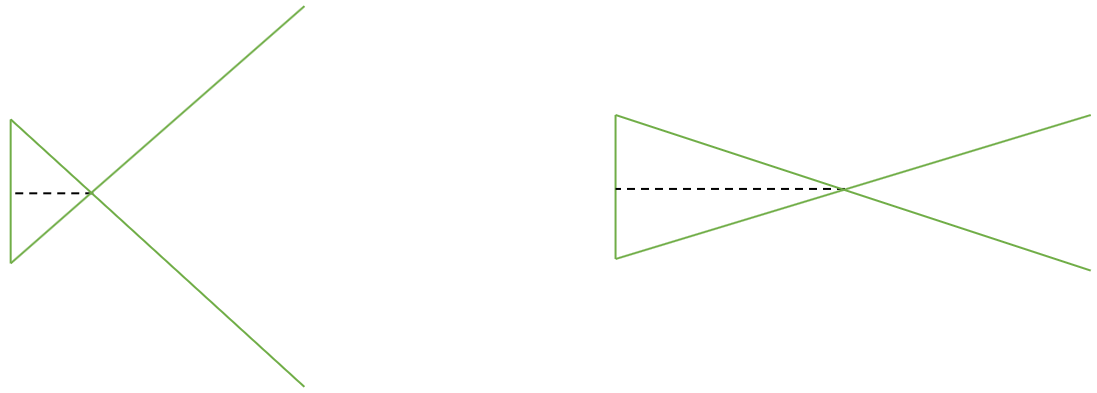
\includegraphics[width=0.4\textwidth]{./img/perspective_projection_proportion.png}
                \caption{Coordinate space by varying focal length}
            \end{figure}
        \end{remark}

        \begin{remark}
            The perspective projection mapping is not a bijection:
            \begin{itemize}
                \item A scene point is mapped into a unique image point.
                \item An image point is mapped onto a 3D line.
            \end{itemize}
            Therefore, reconstructing the 3D structure of a single image is an ill-posed problem (i.e. it has multiple solutions).

            \begin{figure}[H]
                \centering
                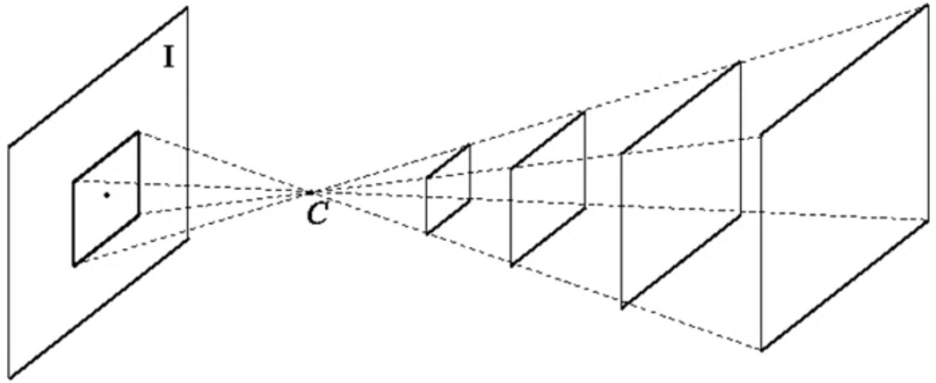
\includegraphics[width=0.3\textwidth]{./img/perspective_projection_loss.png}
                \caption{Projection from scene and image points}
            \end{figure}
        \end{remark}
\end{description}


\subsection{Stereo geometry}

\begin{description}
    \item[Stereo vision] \marginnote{Stereo vision}
        Use multiple images to triangulate the 3D position of an object.
    
    \item[Stereo correspondence] \marginnote{Stereo correspondence}
        Given a point $L$ in an image, find the corresponding point $R$ in another image.

        Without any assumptions, an oracle is needed to determine the correspondences.
\end{description}

\begin{description}
    \item[Standard stereo geometry] \marginnote{Standard stereo geometry}
        Given two reference images, the following assumptions must hold:
        \begin{itemize}
            \item The $X$, $Y$, $Z$ axes are parallel. 
            \item The cameras that took the two images have the same focal length $f$ (coplanar image planes) and 
                the images have been taken at the same time.
            \item There is a horizontal translation $b$ between the two cameras (baseline).
            \item The disparity $d$ is the difference of the $U$ coordinates of the object in the left and right image.
        \end{itemize}

        \begin{theorem}[Fundamental relationship in stereo vision] \marginnote{Fundamental relationship in stereo vision}
            If the assumptions above hold, the following equation holds:
            \[ z = b\frac{f}{d} \]

            \begin{proof}
                Let $P_L = \begin{pmatrix}x_L & y & z\end{pmatrix}$ and $P_R = \begin{pmatrix}x_R & y & z\end{pmatrix}$ be the
                coordinates of the object $P$ with respect to the left and right camera reference system, respectively.
                Let $p_L = \begin{pmatrix}u_L & v\end{pmatrix}$ and $p_R = \begin{pmatrix}u_R & v\end{pmatrix}$ 
                be the coordinates of the object $P$ in the left and right image plane, respectively.
                
                By assumption, we have that $P_L - P_R = \begin{pmatrix} b & 0 & 0 \end{pmatrix}$, where $b$ is the baseline.

                \begin{minipage}{0.6\textwidth}
        
                    By the perspective projection equation, we have that:
                    \[ u_L = x_L\frac{f}{z} \hspace{3em} u_R = x_R\frac{f}{z} \]
                    Disparity is computed as follows:
                    \[ d = u_L - u_R = x_L\frac{f}{z} - x_R\frac{f}{z} = b\frac{f}{z} \]
                    We can therefore obtain the $Z$ coordinate of $P$ as:
                    \[ z = b\frac{f}{d} \]
                \end{minipage}
                \begin{minipage}{0.3\textwidth}
                    \begin{center}
                        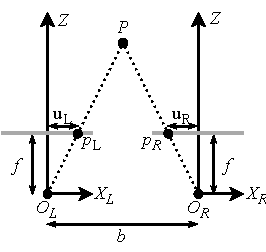
\includegraphics[width=\textwidth]{./img/_standard_stereo_geometry.pdf}
                    \end{center}
                    Note: the $Y$/$V$ axes are not in figure.
                \end{minipage}\\
            \end{proof}

            \begin{remark}
                Disparity and depth are inversely proportional:
                the disparity of two points decreases if the points are farther in depth.
            \end{remark}
        \end{theorem}

        \begin{description}
            \item[Stereo matching] \marginnote{Stereo matching}
                If the assumptions for standard stereo geometry hold,
                to find the object corresponding to $p_L$ in another image, 
                it is sufficient to search along the horizontal axis of $p_L$ looking for the same colors or patterns.

                \begin{figure}[H]
                    \centering
                    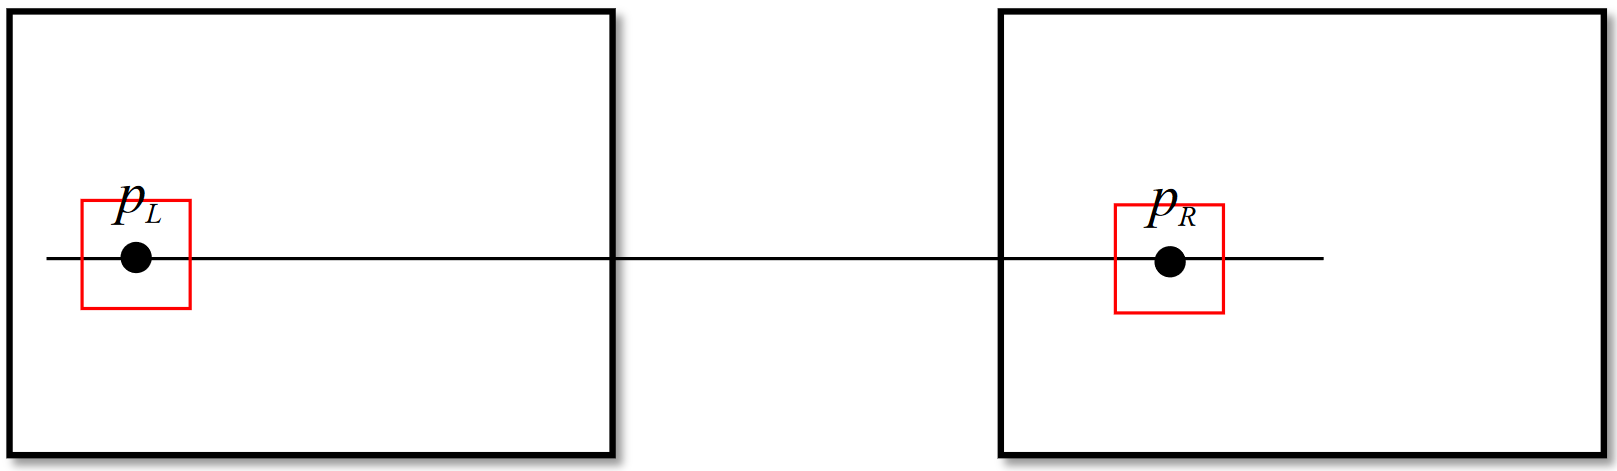
\includegraphics[width=0.5\textwidth]{./img/stereo_matching.png}
                    \caption{Example of stereo matching}
                \end{figure}
        \end{description}

    \item[Epipolar geometry] \marginnote{Epipolar geometry}
        Approach applied when the two cameras are no longer aligned according to the standard stereo geometry assumption.
        Still, the focal lengths and the roto-translation between the two cameras must be known.

        Given two images, we can project the epipolar line related to the point $p_L$ in the left plane onto the right plane
        to reduce the problem of correspondence search to a single dimension.

        \begin{figure}[H]
            \centering
            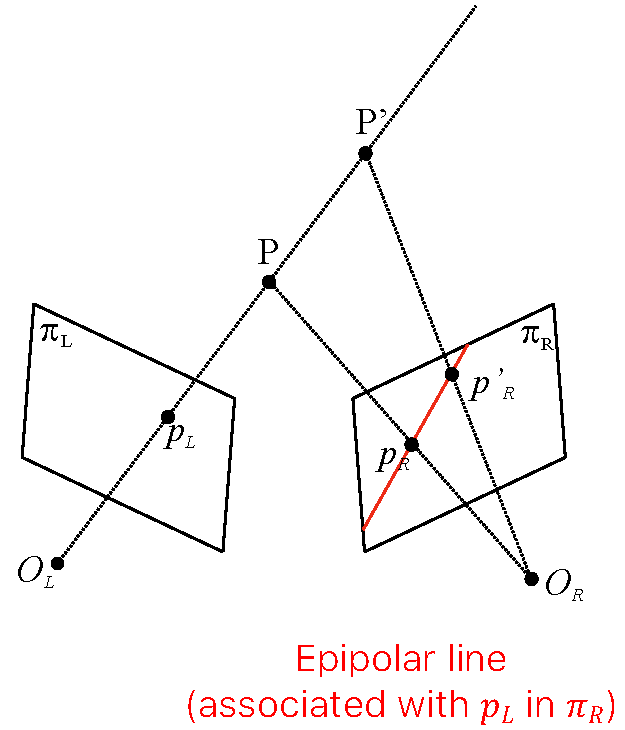
\includegraphics[width=0.3\textwidth]{./img/_epipolar_geometry.pdf}
            \caption{Example of epipolar geometry}
        \end{figure}

        \begin{remark}
            It is nearly impossible to project horizontal epipolar lines and 
            searching through oblique lines is awkward and computationally less efficient than straight lines.
        \end{remark}

        \begin{description}
            \item[Rectification] \marginnote{Rectification}
                Transformation applied to convert epipolar geometry to a standard stereo geometry.
                \begin{figure}[H]
                    \centering
                    \begin{subfigure}{0.35\linewidth}
                        \centering
                        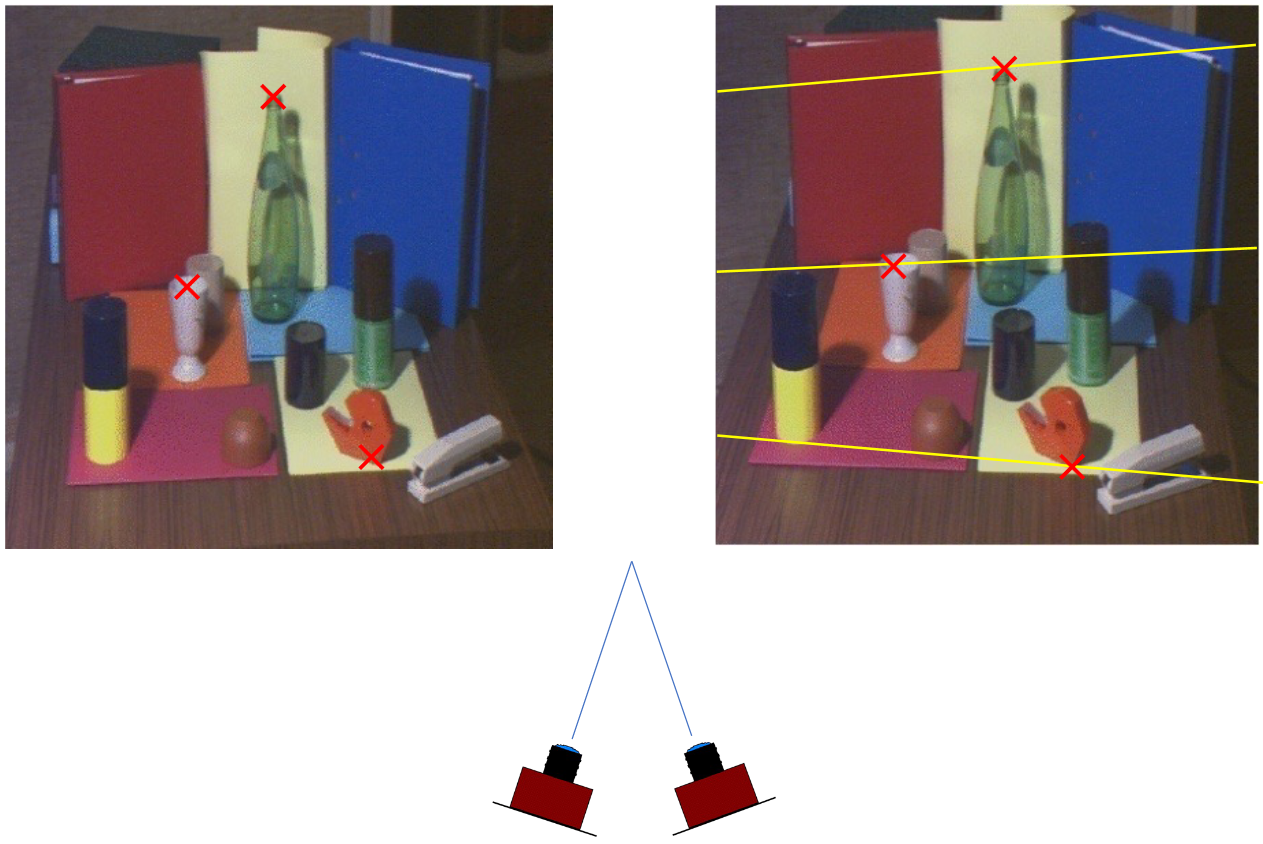
\includegraphics[width=\linewidth]{./img/rectification_no.png}
                        \caption{Images before rectification}
                    \end{subfigure}
                    \begin{subfigure}{0.35\linewidth}
                        \centering
                        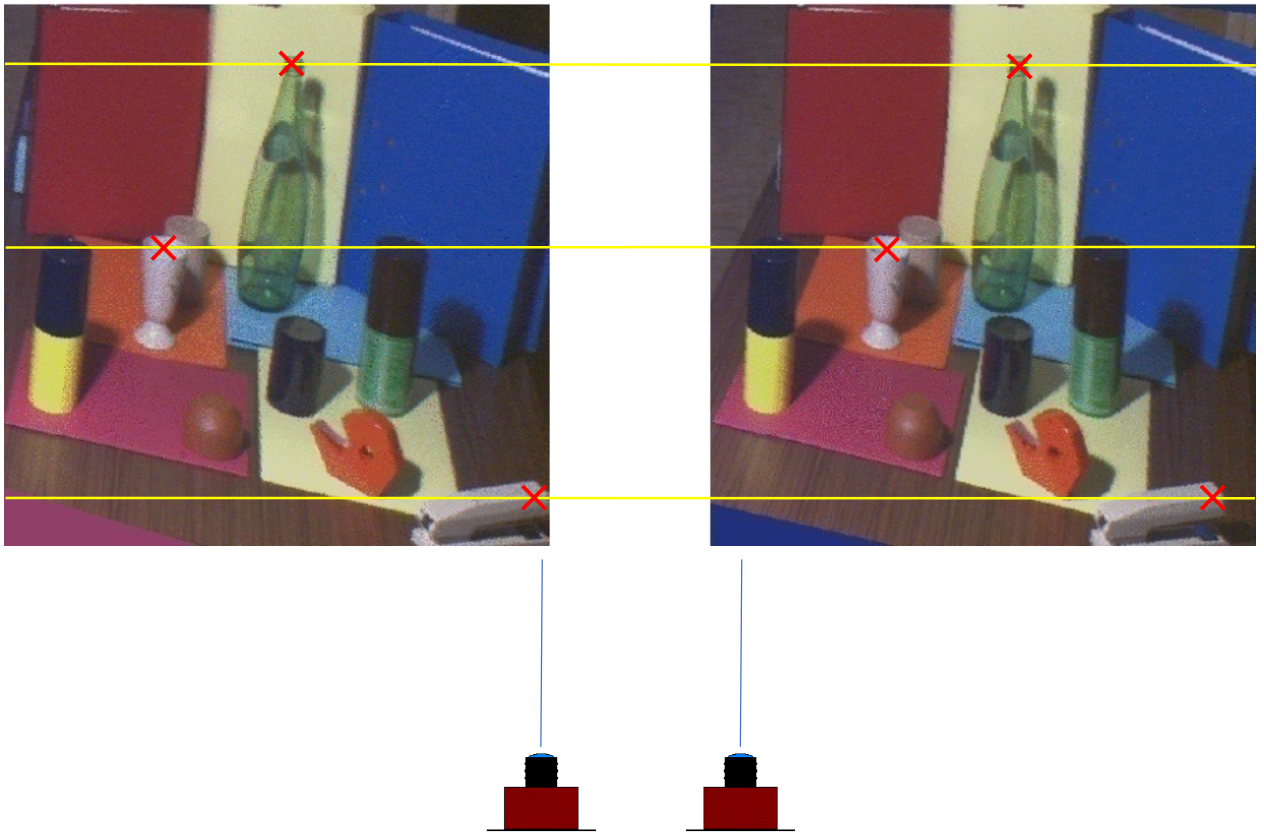
\includegraphics[width=\linewidth]{./img/rectification_yes.png}
                        \caption{Images after rectification}
                    \end{subfigure}
                \end{figure}
        \end{description}
\end{description}


\subsection{Ratios and parallelism}

Given a 3D line of length $L$ lying in a plane parallel to the image plane at distance $z$,
then its length $l$ in the image plane is:
\[ l = L\frac{f}{z} \]

In all the other cases (i.e. when the line is not parallel to the image plane), 
the ratios of lengths and the parallelism of lines are not preserved.

\begin{figure}[H]
    \centering
    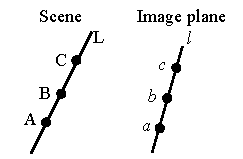
\includegraphics[width=0.25\textwidth]{./img/_perspective_projection_ratio.pdf}
    \caption{Example of not preserved ratios. It holds that $\frac{\overline{AB}}{\overline{BC}} \neq \frac{\overline{ab}}{\overline{bc}}$.}
\end{figure}

\begin{description}
    \item[Vanishing point] \marginnote{Vanishing point}
        Intersection point of lines that are parallel in the scene but not in the image plane.

        \begin{figure}[H]
            \centering
            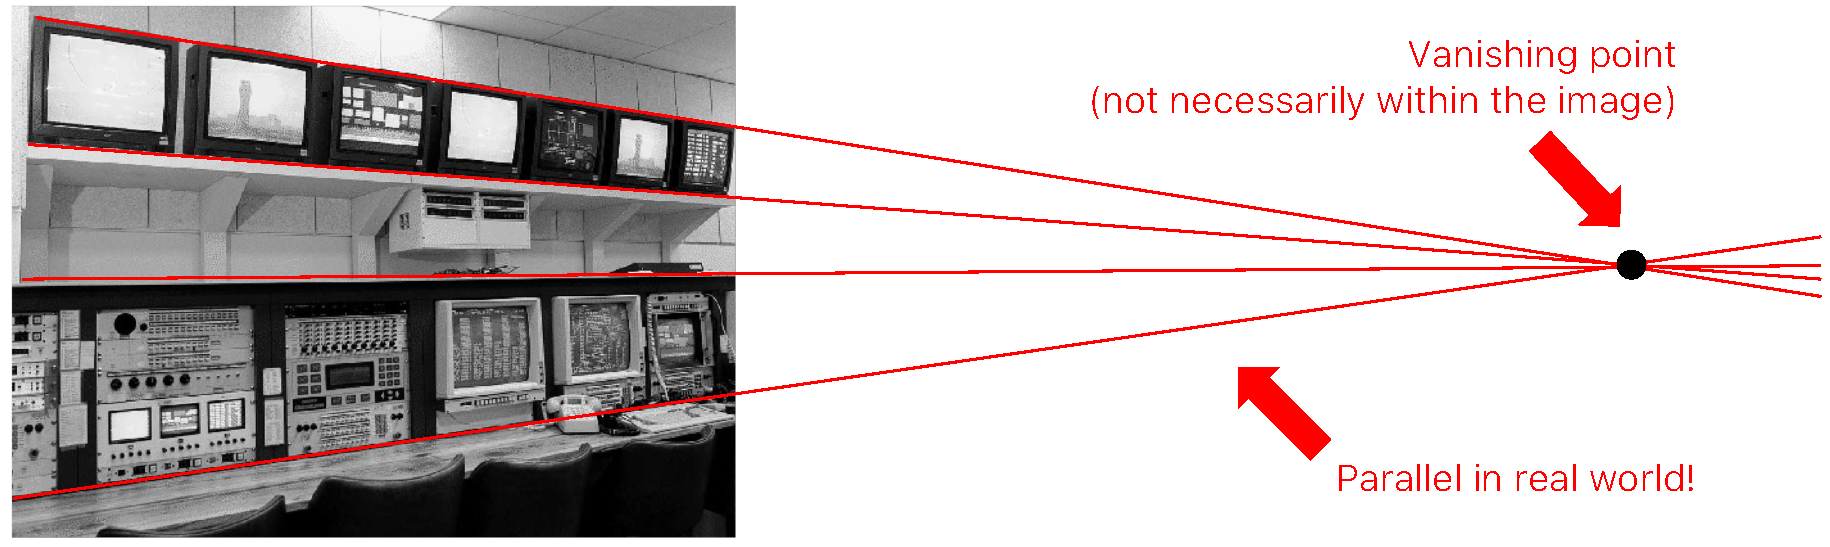
\includegraphics[width=0.6\textwidth]{./img/_vanishing_point.pdf}
            \caption{Example of vanishing point}
        \end{figure}
\end{description}



\section{Lens}

\begin{description}
    \item[Depth of field (DOF)] \marginnote{Depth of field (DOF)}
        Distance at which a scene point is in focus (i.e. when all its light rays gathered by the imaging device hit the image plane at the same point).

        \begin{remark}
            Because of the small size of the aperture, a pinhole camera has infinite depth of field
            but requires a long exposure time making it only suitable for static scenes.
        \end{remark}


    \item[Lens] \marginnote{Lens}
        A lens gathers more light from the scene point and focuses it on a single image point.

        This allows for a smaller exposure time but limits the depth of field (i.e. only a limited range of distances in the image can be in focus at the same time).


    \item[Thin lens] \marginnote{Thin lens}
        Approximate model for lenses.

        \begin{minipage}{0.65\textwidth}
            \begin{description}
                \setlength\itemsep{0em}
                \item[Scene point] $P$ (the object in the real world).
                \item[Image point] $p$ (the object in the image).
                \item[Object--lens distance] $o$.
                \item[Image--lens distance] $i$ (i.e. focal length of the camera).
                \item[Center of the lens] $C$.
                \item[Focal length of the lens] $f$.
                \item[Focal plane/focus of the lens] $F$.
            \end{description}
        \end{minipage}
        \begin{minipage}{0.4\textwidth}
            \centering
            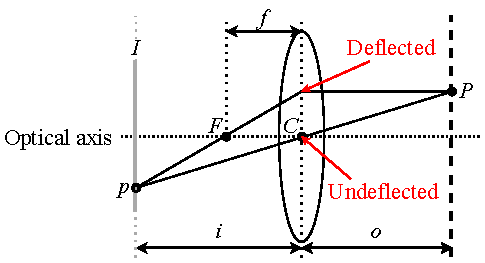
\includegraphics[width=\textwidth]{./img/_thin_lens.pdf}
        \end{minipage}

        A thin lens has the following properties:
        \begin{itemize}
            \item Rays hitting the lens parallel to the optical axis are deflected to pass through the focal plane of the lens $F$.
            \item Rays passing through the center of the lens $C$ are undeflected.
            \item The following equation holds: \marginnote{Thin lens equation}
                \[ \frac{1}{o} + \frac{1}{i} = \frac{1}{f} \] 
        \end{itemize}

    \item[Image formation]
        When the image is in focus, the image formation process follows the normal rules of the perspective projection model where:
        \begin{itemize}
            \item $C$ is the optical center.
            \item $i$ is the focal length of the camera.
        \end{itemize}

        By fixing the focal length of the lens ($f$),
        we can determine the distance of the scene point ($o$) or the image point ($i$) required to have the object in focus.
        \[ \frac{1}{o}+\frac{1}{i} = \frac{1}{f} \iff o = \frac{if}{i - f} \hspace{3em} \frac{1}{o}+\frac{1}{i} = \frac{1}{f} \iff i = \frac{of}{o - f} \]

        \begin{remark}
            Points projected in front or behind the image plane will create a circle of confusion (blur).

            \begin{figure}[H]
                \centering
                \begin{subfigure}{0.3\textwidth}
                    \centering
                    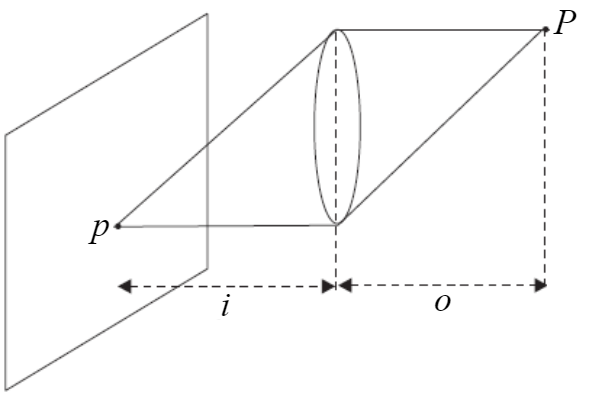
\includegraphics[width=\textwidth]{./img/thin_lens_formation1.png}
                    \caption{Image in focus}
                \end{subfigure}
                \begin{subfigure}{0.3\textwidth}
                    \centering
                    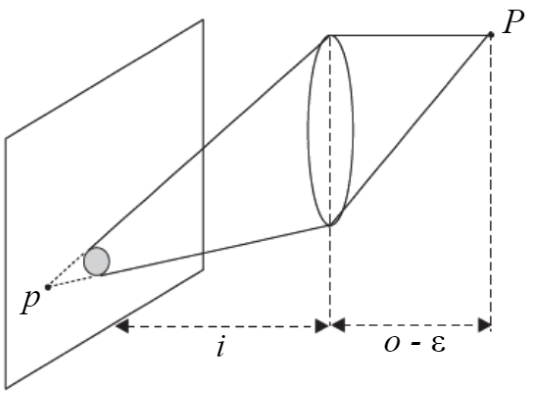
\includegraphics[width=0.8\textwidth]{./img/thin_lens_formation2.png}
                    \caption{Projection behind the image plane}
                \end{subfigure}
                \begin{subfigure}{0.3\textwidth}
                    \centering
                    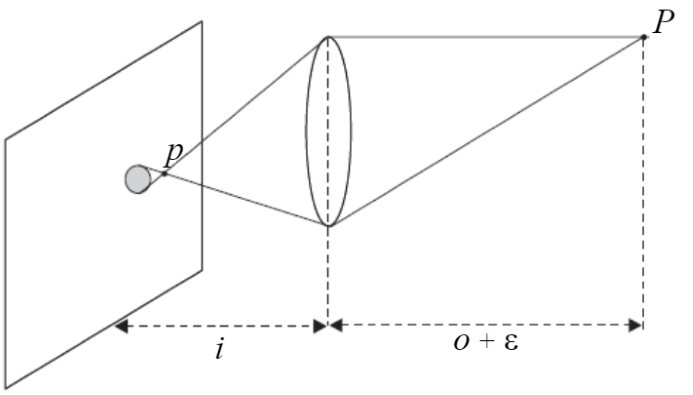
\includegraphics[width=\textwidth]{./img/thin_lens_formation3.png}
                    \caption{Projection in front of the image plane}
                \end{subfigure}
            \end{figure}
        \end{remark}

    \item[Adjustable diaphragm] \marginnote{Adjustable diaphragm}
        Device to control the light gathered by the effective aperture of the lens.

        Reducing the aperture will result in less light and an increased depth of field.

        \begin{remark}
            On a theoretical level, images that are not in focus appear blurred (circles of confusion).
            Despite that, if the circle is smaller than the photo-sensing elements (i.e. pixels), it will appear in focus.
        \end{remark}

    \item[Focusing mechanism] \marginnote{Focusing mechanism}
        Allows the lens to translate along the optical axis to increase its distance to the image plane.

        At the minimum extension (\Cref{fig:focus_mechanism_min}), we have that:
            \[ i = f \text{ and } o = \infty \text{ as the thin lens equation states that } \frac{1}{o} + \frac{1}{i} = \frac{1}{f} \]
        By increasing the extension (i.e. increase $i$), we have that the distance to the scene point $o$ decreases.
        The maximum extension determines the minimum focusing distance.

            
        \begin{figure}[H]
            \centering
            \begin{subfigure}{0.4\textwidth}
                \centering
                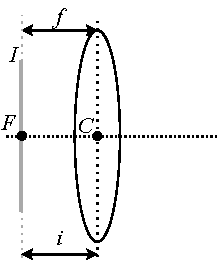
\includegraphics[width=0.45\textwidth]{./img/_focus_mechanism1.pdf}
                \caption{Minimum extension} \label{fig:focus_mechanism_min}
            \end{subfigure}
            \begin{subfigure}{0.4\textwidth}
                \centering
                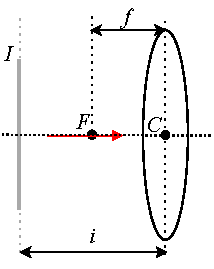
\includegraphics[width=0.45\textwidth]{./img/_focus_mechanism2.pdf}
                \caption{Maximum extension} \label{fig:focus_mechanism_max}
            \end{subfigure}
            \caption{Extension of a focusing mechanism}
        \end{figure}
\end{description}



\section{Image digitalization}


\subsection{Sampling and quantization}

The image plane of a camera converts the received irradiance into electrical signals.

\begin{figure}[H]
    \centering
    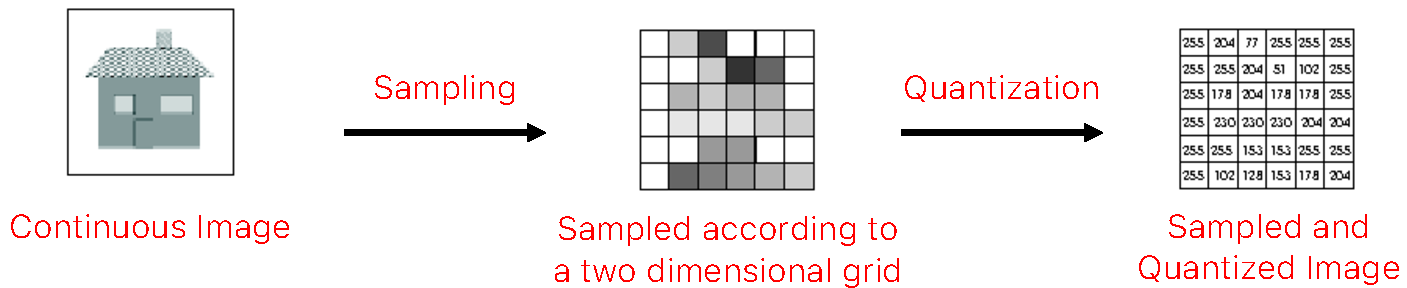
\includegraphics[width=0.6\textwidth]{./img/_digitalization.pdf}
    \caption{Image digitalization steps}
\end{figure}

\begin{description}
    \item[Sampling] \marginnote{Sampling} 
        The continuous electrical signal is sampled to produce a $N \times M$ matrix of pixels:
        \[ 
            I(x, y) = \begin{pmatrix}
                I(0, 0) & \hdots & I(0, M-1) \\
                \vdots & \ddots & \vdots \\
                I(N-1, 0) & \hdots & I(N-1, M-1) \\
            \end{pmatrix}    
        \]

    \item[Quantization] \marginnote{Quantization}
        Let $m$ be the number of bits used to encode a pixel.
        The value of each pixel is quantized into $2^m$ discrete gray levels.
        
        \begin{remark}
            A grayscale image usually uses $8$ bits

            An RGB image usually uses $3 \cdot 8$ bits.
        \end{remark}
\end{description}

\begin{remark}
    The more bits are used for the representation, the higher the quality of the image will be.
    \begin{itemize}
        \item Sampling with fewer bits will result in a lower resolution (aliasing).
        \item Quantization with fewer bits will result in less representable colors.
    \end{itemize}
    \begin{figure}[H]
        \centering
        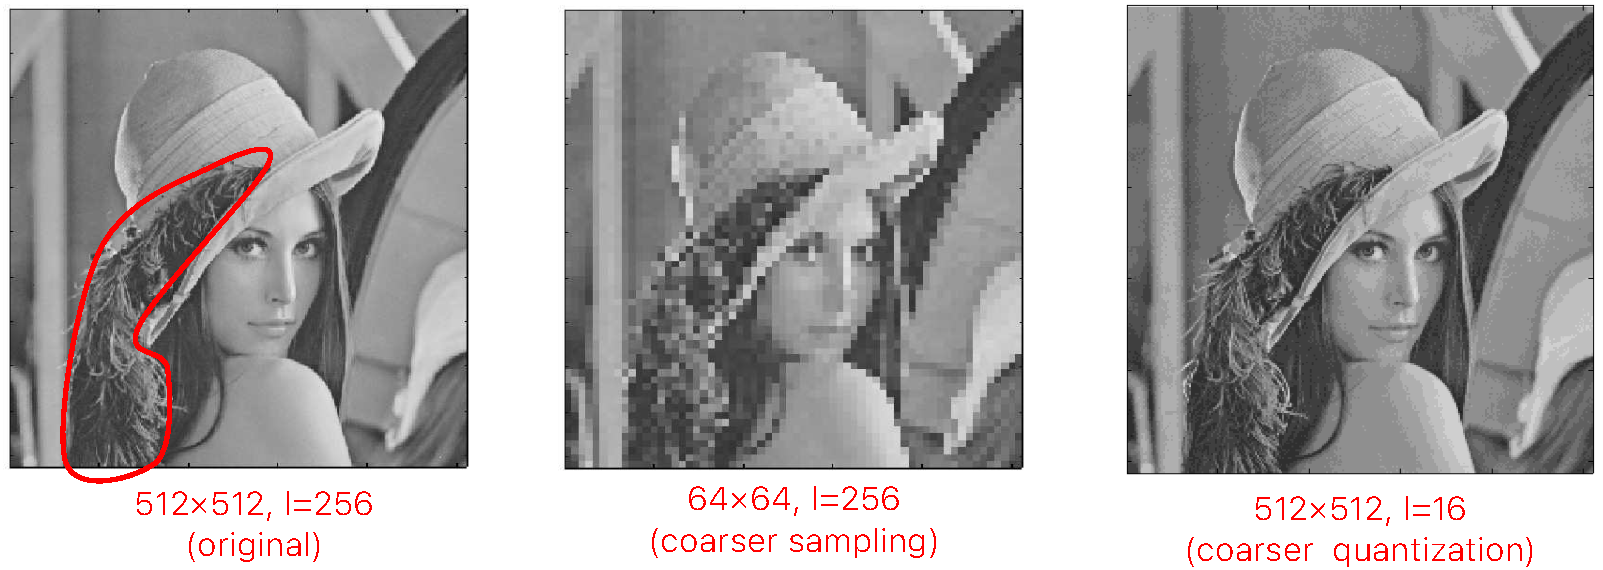
\includegraphics[width=0.6\textwidth]{./img/_digitalization_quality.pdf}
        \caption{Sampling and quantization using fewer bits}
    \end{figure}
\end{remark}


\subsection{Camera sensors}

\begin{description}
    \item[Photodetector] \marginnote{Photodetector}
        Sensor that, during the exposure time, converts the light into a proportional electrical charge that 
        will be processed by a circuit and converted into a digital or analog signal.

        \begin{figure}[H]
            \centering
            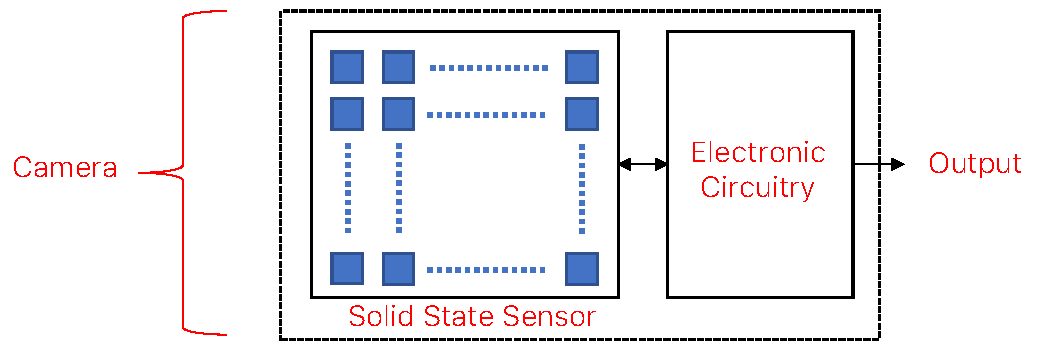
\includegraphics[width=0.55\textwidth]{./img/_camera_sensors.pdf}
            \caption{Components of a camera}
        \end{figure}

        The two main sensor technologies are:
        \begin{descriptionlist}
            \item[Charge Coupled Device (CCD)] \marginnote{Charge Coupled Device (CCD)}
                Typically produces higher quality images but are more expensive.

            \item[Complementary Metal Oxide Semiconductor (CMOS)] \marginnote{Complementary Metal Oxide Semiconductor (CMOS)}
                Generally produces lower quality images but is more compact and less expensive.
                Each sensor has integrated its own circuitry that allows to read an arbitrary window of the sensors.
        \end{descriptionlist}

    \item[Color sensors] \marginnote{Color sensors}
        CCD and CMOS sensors are sensitive to a wide spectrum of light frequencies (both visible and invisible) but
        are unable to sense colors as they produce a single value per pixel.

        \begin{figure}[H]
            \centering
            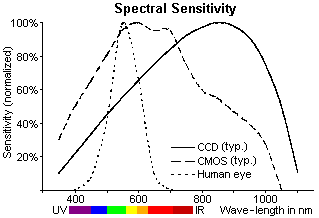
\includegraphics[width=0.35\textwidth]{./img/sensors_sensitivity.png}
            \caption{CCD and CMOS spectral sensitivity}
        \end{figure}

        \begin{description}
            \item[Color Filter Array (CFA)] \marginnote{Color Filter Array (CFA)}
                Filter placed in front of a photodetector to allow it to detect colors.

                Possible approaches are:
                \begin{descriptionlist}
                    \item[Bayer CFA] 
                        A grid of green, blue, and red filters with the greens being twice as much as the others (the human eye is more sensible to the green range).
                        To determine the RGB value of each pixel, missing color channels are sampled from neighboring pixels (demosaicking).
                        
                        \begin{figure}[H]
                            \centering
                            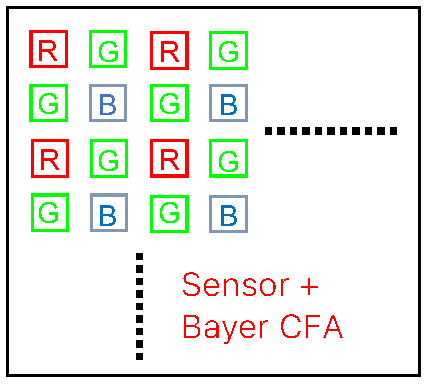
\includegraphics[width=0.15\textwidth]{./img/_bayer_cfa.pdf}
                            \caption{Example of Bayer filter}
                        \end{figure}

                    \item[Optical prism] 
                        A prism splits the incoming light into 3 RGB beams, each directed to a different sensor.
                        It is more expensive than Bayer CFA.
                \end{descriptionlist}
        \end{description}
\end{description}


\subsection{Metrics}

\begin{description}
    \item[Signal to Noise Ratio (SNR)] \marginnote{Signal to Noise Ratio (SNR)}
        Quantifies the strength of the actual signal with respect to unwanted noise.

        Sources of noise are:
        \begin{descriptionlist}
            \item[Photon shot noise] Number of photons captured during exposure time.
            \item[Elecronic circuitry noise] Generated by the electronics that read the sensors.
            \item[Quantization noise] Caused by the digitalization of the image (ADC conversion).
            \item[Dark current noise] Random charge caused by thermal excitement.
        \end{descriptionlist}

        SNR is usually expressed in decibels or bits:
        \[ \texttt{SNR}_\text{db} = 20 \cdot \log_{10}(\texttt{SNR}) \hspace{3em} \texttt{SNR}_\text{bit} = \log_{2}(\texttt{SNR}) \]

    \item[Dynamic Range (DR)] \marginnote{Dynamic Range (DR)}
        Measures the ability of a sensor to capture both the dark and bright structure of the scene.

        Let:
        \begin{itemize}
            \item $E_\text{min}$ be the minimum detectable irradiation. This value depends on the noise.
            \item $E_\text{max}$ be the saturation irradiation (i.e. the maximum amount of light that fills the capacity of the photodetector).
        \end{itemize}
        DR is defined as:
        \[ \texttt{DR} = \frac{E_\text{max}}{E_\text{mix}} \]
        As with SNR, DR can be expressed in decibels or bits.
\end{description}